\section{Introduction}
\vspace{0.2in}
\hspace*{0.16in}
In this chapter, we will present artificial intelligence with all of its branches, and then dive deeper into convolutional neural networks (CNNs) and their layers. Finally, we will present some CNN architectures and image processing methods.

\section{Artificial Intelligence}
\subsection{Definition}
It is the science and engineering of making intelligent machines, especially intelligent computer programs. It is related to the similar task of using computers to understand human intelligence, but AI does not have to confine itself to methods that are biologically observable. \textsuperscript{\cite{mccarthy2004artificial}}

Artificial intelligence algorithms can be categorised into these four main types:

\begin{itemize}
    \item \textbf{Supervised learning:}
        Supervised learning, as the name indicates, has the presence of a supervisor as a teacher. Basically supervised learning is when we teach or train the machine using data that is well labeled. Which means some data is already tagged with the correct answer. After that, the machine is provided with a new set of examples (data) so that the supervised learning algorithm analyses the training data (set of training examples) and produces a correct outcome from labeled data. \textsuperscript{\cite{AITypes-GeeksForGeeks}}
    \item \textbf{Unsupervised learning:}
        Unsupervised learning is the training of a machine using information that is neither classified nor labeled and allowing the algorithm to act on that information without guidance. Here the task of the machine is to group unsorted information according to similarities, patterns, and differences without any prior training of data. \textsuperscript{\cite{AITypes-GeeksForGeeks}}
    \item \textbf{Semi Supervised learning:}
    \item \textbf{Reinforcement learning:}
\end{itemize}

\vspace{0.2in}

\begin{table}[H]
\centering
\resizebox{\textwidth}{!}{%
\begin{tabular}{|
>{\columncolor[HTML]{FFFFFF}}c |
>{\columncolor[HTML]{FFFFFF}}c |
>{\columncolor[HTML]{FFFFFF}}c 
>{\columncolor[HTML]{FFFFFF}}l 
>{\columncolor[HTML]{FFFFFF}}l |}
\hline
\textbf{Parameters}               & \textbf{Supervised machine learning} & \multicolumn{3}{c|}{\cellcolor[HTML]{FFFFFF}\textbf{Unsupervised machine learning}} \\ \hline
\textbf{Input Data} &
  \begin{tabular}[c]{@{}c@{}}Algorithms are trained\\ using labeled data.\end{tabular} &
  \multicolumn{3}{c|}{\cellcolor[HTML]{FFFFFF}\begin{tabular}[c]{@{}c@{}}Algorithms are used against\\ data that is not labeled\end{tabular}} \\ \hline
\textbf{Computational Complexity} & Simpler method                       & \multicolumn{3}{c|}{\cellcolor[HTML]{FFFFFF}Computationally complex}                \\ \hline
\textbf{Accuracy}                 & Highly accurate                      & \multicolumn{3}{c|}{\cellcolor[HTML]{FFFFFF}Less accurate}                          \\ \hline
\end{tabular}%
}
\caption{Table that presents diffrence between supervised and unsupervised machine learning \textsuperscript{\cite{AITypes-GeeksForGeeks}}}
\label{Table that presents diffrence between supervised and unsupervised machine learning}
\end{table}


\subsection{Machine Learning}
Machine learning is a branch of artificial intelligence (AI) and computer science which focuses on the use of data and algorithms to imitate the way that humans learn, gradually improving its accuracy. \textsuperscript{\cite{ML-IBM}}

\begin{itemize}
  \item \textbf{Linear Regression:}
      Linear Regression is a machine learning algorithm based on supervised learning. It performs a regression task. Regression models a target prediction value based on independent variables. It is mostly used for finding out the relationship between variables and forecasting. Different regression models differ based on – the kind of relationship between dependent and independent variables they are considering, and the number of independent variables getting used. \textsuperscript{\cite{LR-GeeksForGeeks}}
  \item \textbf{Support Vector Machines:}
      Support Vector Machine (SVM) is a computer algorithm that learns by example to assign labels to objects. \textsuperscript{\cite{boser1992training}} For instance, an SVM can learn to recognize fraudulent credit card activity by examining hundreds or thousands of fraudulent and nonfraudulent credit card activity reports. Alternatively, an SVM can learn to recognize handwritten digits by examining a large collection of scanned images of handwritten zeroes, ones and so fourth. \textsuperscript{\cite{noble2006support}}
  \item \textbf{Gradient Descent:}
      Gradient descent is an optimization algorithm used to minimize some function by iteratively moving in the direction of steepest descent as defined by the negative of the gradient. In machine learning, we use gradient descent to update the parameters of our model. Parameters refer to coefficients in Linear Regression and weights in neural networks. \textsuperscript{\cite{DG-ml-cheatsheet}}
\end{itemize}

\subsection{Deep Learning}
\subsubsection{Neural Networks}
\subsubsection{Convolutional Neural Networks}
CNNs or ConvNets are among the most successful and widely used architectures in the deep learning community, especially for computer vision tasks . CNNs were initially proposed by Fukushima in his seminal paper on the “Neocognitron” \textsuperscript{\cite{fukushima_Neocognitron}}.

\begin{figure}[H]
\centering
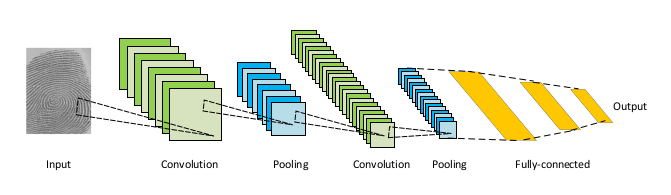
\includegraphics[width=\linewidth]{../images/CNN.png}
\caption{Architecture of convolutional neural networks. From \textsuperscript{\cite{minaee2021image}}}
\label{fig:CNN}
\end{figure}

Convolutional neural networks are distinguished from other neural networks by their superior performance with image, speech, or audio signal inputs. They have three main types of layers, which are:

\begin{itemize}
    \item Convolutional layer
    \item Pooling layer
    \item Fully-connected (FC) layer
\end{itemize}

The convolutional layer is the first layer of a convolutional network. While convolutional layers can chained by additional convolutional layers or pooling layers, the fully-connected layer is the final layer. With each layer, the CNN increases in its complexity, identifying greater portions of the image. Earlier layers focus on simple features, such as colors and edges. As the image data progresses through the layers of the CNN, it starts to recognize larger elements or shapes of the object until it finally identifies the intended object. 
    
    
\begin{enumerate}
    \item \textbf{Convolutional layer} : \\
        The convolutional layer is the core building block of a CNN, and it is where the majority of computation occurs. It requires a few components, which are input data, a filter, and will output a feature map. Let’s assume that the input will be a color image, which is made up of a matrix of pixels in 3D. This means that the input will have three dimensions—a height, width, and depth—which correspond to RGB in an image. We also have a feature detector, also known as a kernel or a filter, which will move across the receptive fields of the image, checking if the feature is present. This process is known as a convolution. \textsuperscript{\cite{CNN-IBM}} \\
        The feature detector is a two-dimensional (2-D) array of weights, which represents part of the image. While they can vary in size, the filter size is typically a 3x3 matrix; this also determines the size of the receptive field. The filter is then applied to an area of the image, and a dot product is calculated between the input pixels and the filter. This dot product is then fed into an output array. Afterwards, the filter shifts by a stride, repeating the process until the kernel has swept across the entire image. The final output from the series of dot products from the input and the filter is known as a feature map, activation map, or a convolved feature.
        \begin{figure}[H]
            \centering
            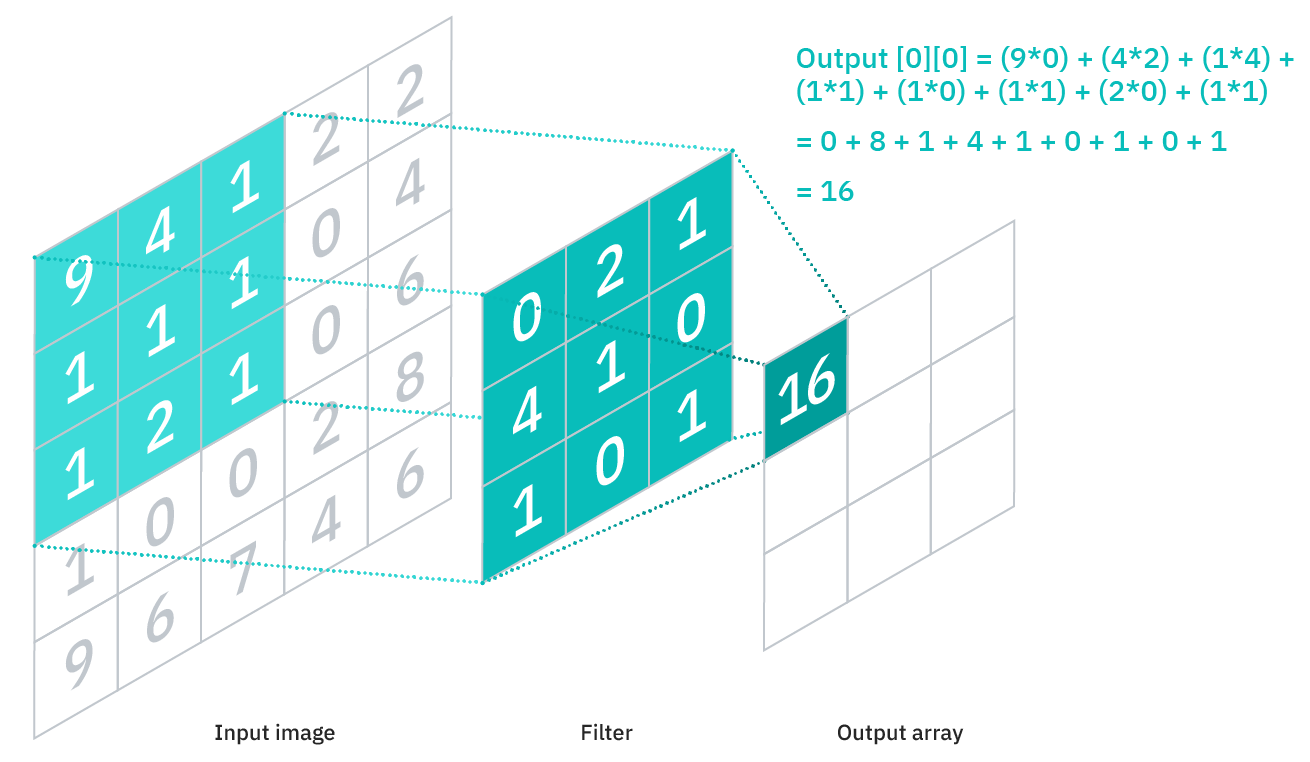
\includegraphics[width=10cm]{../images/CNN-kernel.png}
            \caption{CNN kernel}
            \label{fig:CNN-kernel}
        \end{figure}
        as we can see in the fig \ref{fig:CNN-kernel}, the kernel will browse all the matrix by shifting it's position. where the weights in the kernel will remain fixed as it moves across the image, which is also known as parameter sharing. Some parameters, like the weight values, adjust during training through the process of backpropagation and gradient descent. However, there are three hyperparameters which affect the volume size of the output that need to be set before the training of the neural network begins. These include:
        \begin{itemize}
            \item \textbf{The number of filters} affects the depth of the output. For example, three distinct filters will give us three different feature maps, creating a depth of three.
            \item \textbf{Stride} is the distance, or number of pixels, that the kernel moves over the input matrix. While stride values of two or greater is rare, a larger stride yields a smaller output.
            \item \textbf{Zero-padding }is usually used when the filters do not fit the input image. This sets all elements that fall outside of the input matrix to zero, producing a larger or equally sized output. There are three types of padding:
            \begin{itemize}
                \item \textbf{Valid padding}: This is also known as no padding. In this case, the last convolution is dropped if dimensions do not align.
                \item \textbf{Same padding}: This padding ensures that the output layer has the same size as the input layer
                \item \textbf{Full padding}: This type of padding increases the size of the output by adding zeros to the border of the input.
            \end{itemize}
        \end{itemize}
        
        \begin{figure}[H]
            \centering
            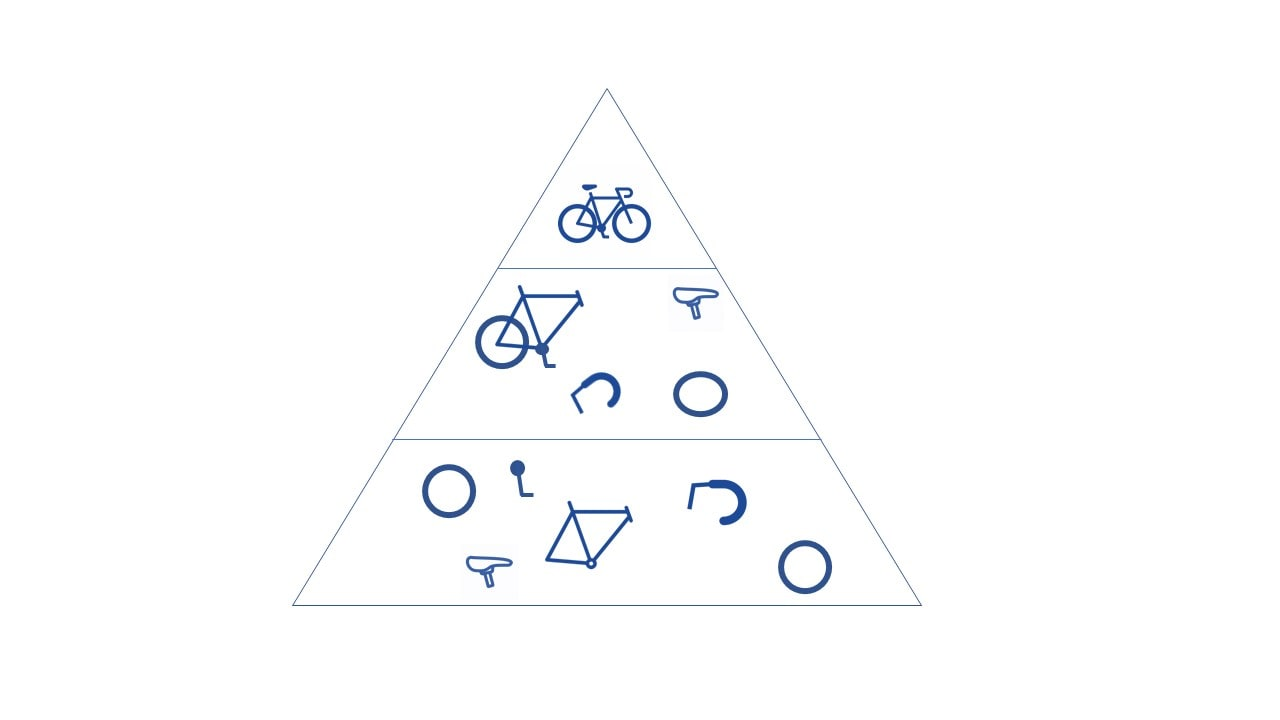
\includegraphics[width=10cm]{../images/CNN-Feature-Hierarchy.jpg}
            \caption{Feature Hierarchy}
            \label{fig:CNN-Feature-Hierarchy}
        \end{figure}
        
        After each convolution operation, a CNN applies an activation function to the feature map, the most used activation function is the Rectified Linear Unit (ReLU).\\
        As we mentioned earlier, when we chain convolutional layers, the structure of the CNN can become hierarchical as the later layers can see the pixels within the receptive fields of prior layers.  As an example, let’s assume that we’re trying to determine if an image contains a bicycle. You can think of the bicycle as a sum of parts. It is comprised of a frame, handlebars, wheels, pedals, et cetera. Each individual part of the bicycle makes up a lower-level pattern in the neural net, and the combination of its parts represents a higher-level pattern, creating a feature hierarchy within the CNN.
    \item \textbf{Pooling Layer}:\\
        Pooling layers, also known as downsampling, conducts dimensionality reduction, reducing the number of parameters in the input. Similar to the convolutional layer, the pooling operation sweeps a filter across the entire input, but the difference is that this filter does not have any weights. Instead, the kernel applies an aggregation function to the values within the receptive field, populating the output array. There are two main types of pooling:
        \begin{itemize}
            \item \textbf{Max pooling}: As the filter moves across the input, it selects the pixel with the maximum value to send to the output array. As an aside, this approach tends to be used more often compared to average pooling.
            \item \textbf{Average pooling}: As the filter moves across the input, it calculates the average value within the receptive field to send to the output array.
        \end{itemize}
        
        While a lot of information is lost in the pooling layer, it also has a number of benefits to the CNN. They help to reduce complexity, improve efficiency, and limit risk of overfitting.
    
    \item \textbf{Fully-Connected Layer}:\\
        The name of the fully-connected layer aptly describes itself. The pixel values of the input image are not directly connected to the output layer in partially connected layers. However, in the fully-connected layer, each node in the output layer connects directly to a node in the previous layer.

        This layer performs the task of classification based on the features extracted through the previous layers and their different filters. While convolutional and pooling layers tend to use ReLu functions or other activation functions, FC layers usually leverage a softmax or sigmoid activation function to classify inputs appropriately, producing a probability from 0 to 1.
        
\end{enumerate}


\section{CNN architectures}
\vspace{0.2in}
\hspace*{0.16in}

\section{Image Processing Methods}
\vspace{0.2in}
\hspace*{0.16in}
